\documentclass[english]{article}

\usepackage{graphicx}
\usepackage{grffile}
\usepackage[T1]{fontenc}
\usepackage{babel}
\usepackage{wrapfig}
\usepackage{hyperref}

\date{\today}

\graphicspath{{Pictures/}}
\begin{document}	
	\begin{titlepage}
		\pagenumbering{gobble}
		\begin{figure}[!t]
			
\includegraphics[width=\linewidth]{up_logo.png}
		\end{figure}
		\vspace*{\stretch{1.0}}
		\begin{center}
			\huge{Project: GENERIC PROJECT}\\
			\large{Client: GENERIC CLIENT}\\
			\vspace{10mm}
			\huge{Team: A-Cube-N}\\
		\end{center}
		\begin{center}
			\begin{tabular}{ c c c }
				Dunkley, Nathan & Grobler, Arno & Lochner, Amy \\
				\texttt{14145759} & \texttt{14011396} & \texttt{14038600}\\
				& Maree, Armand &\\
				& \texttt{12017800} &
			\end{tabular}
		\end{center}
		\begin{center}
			Department of Computer Science, University of Pretoria
		\end{center}
		\begin{center}
			\today
			\begin{figure}[!h]
				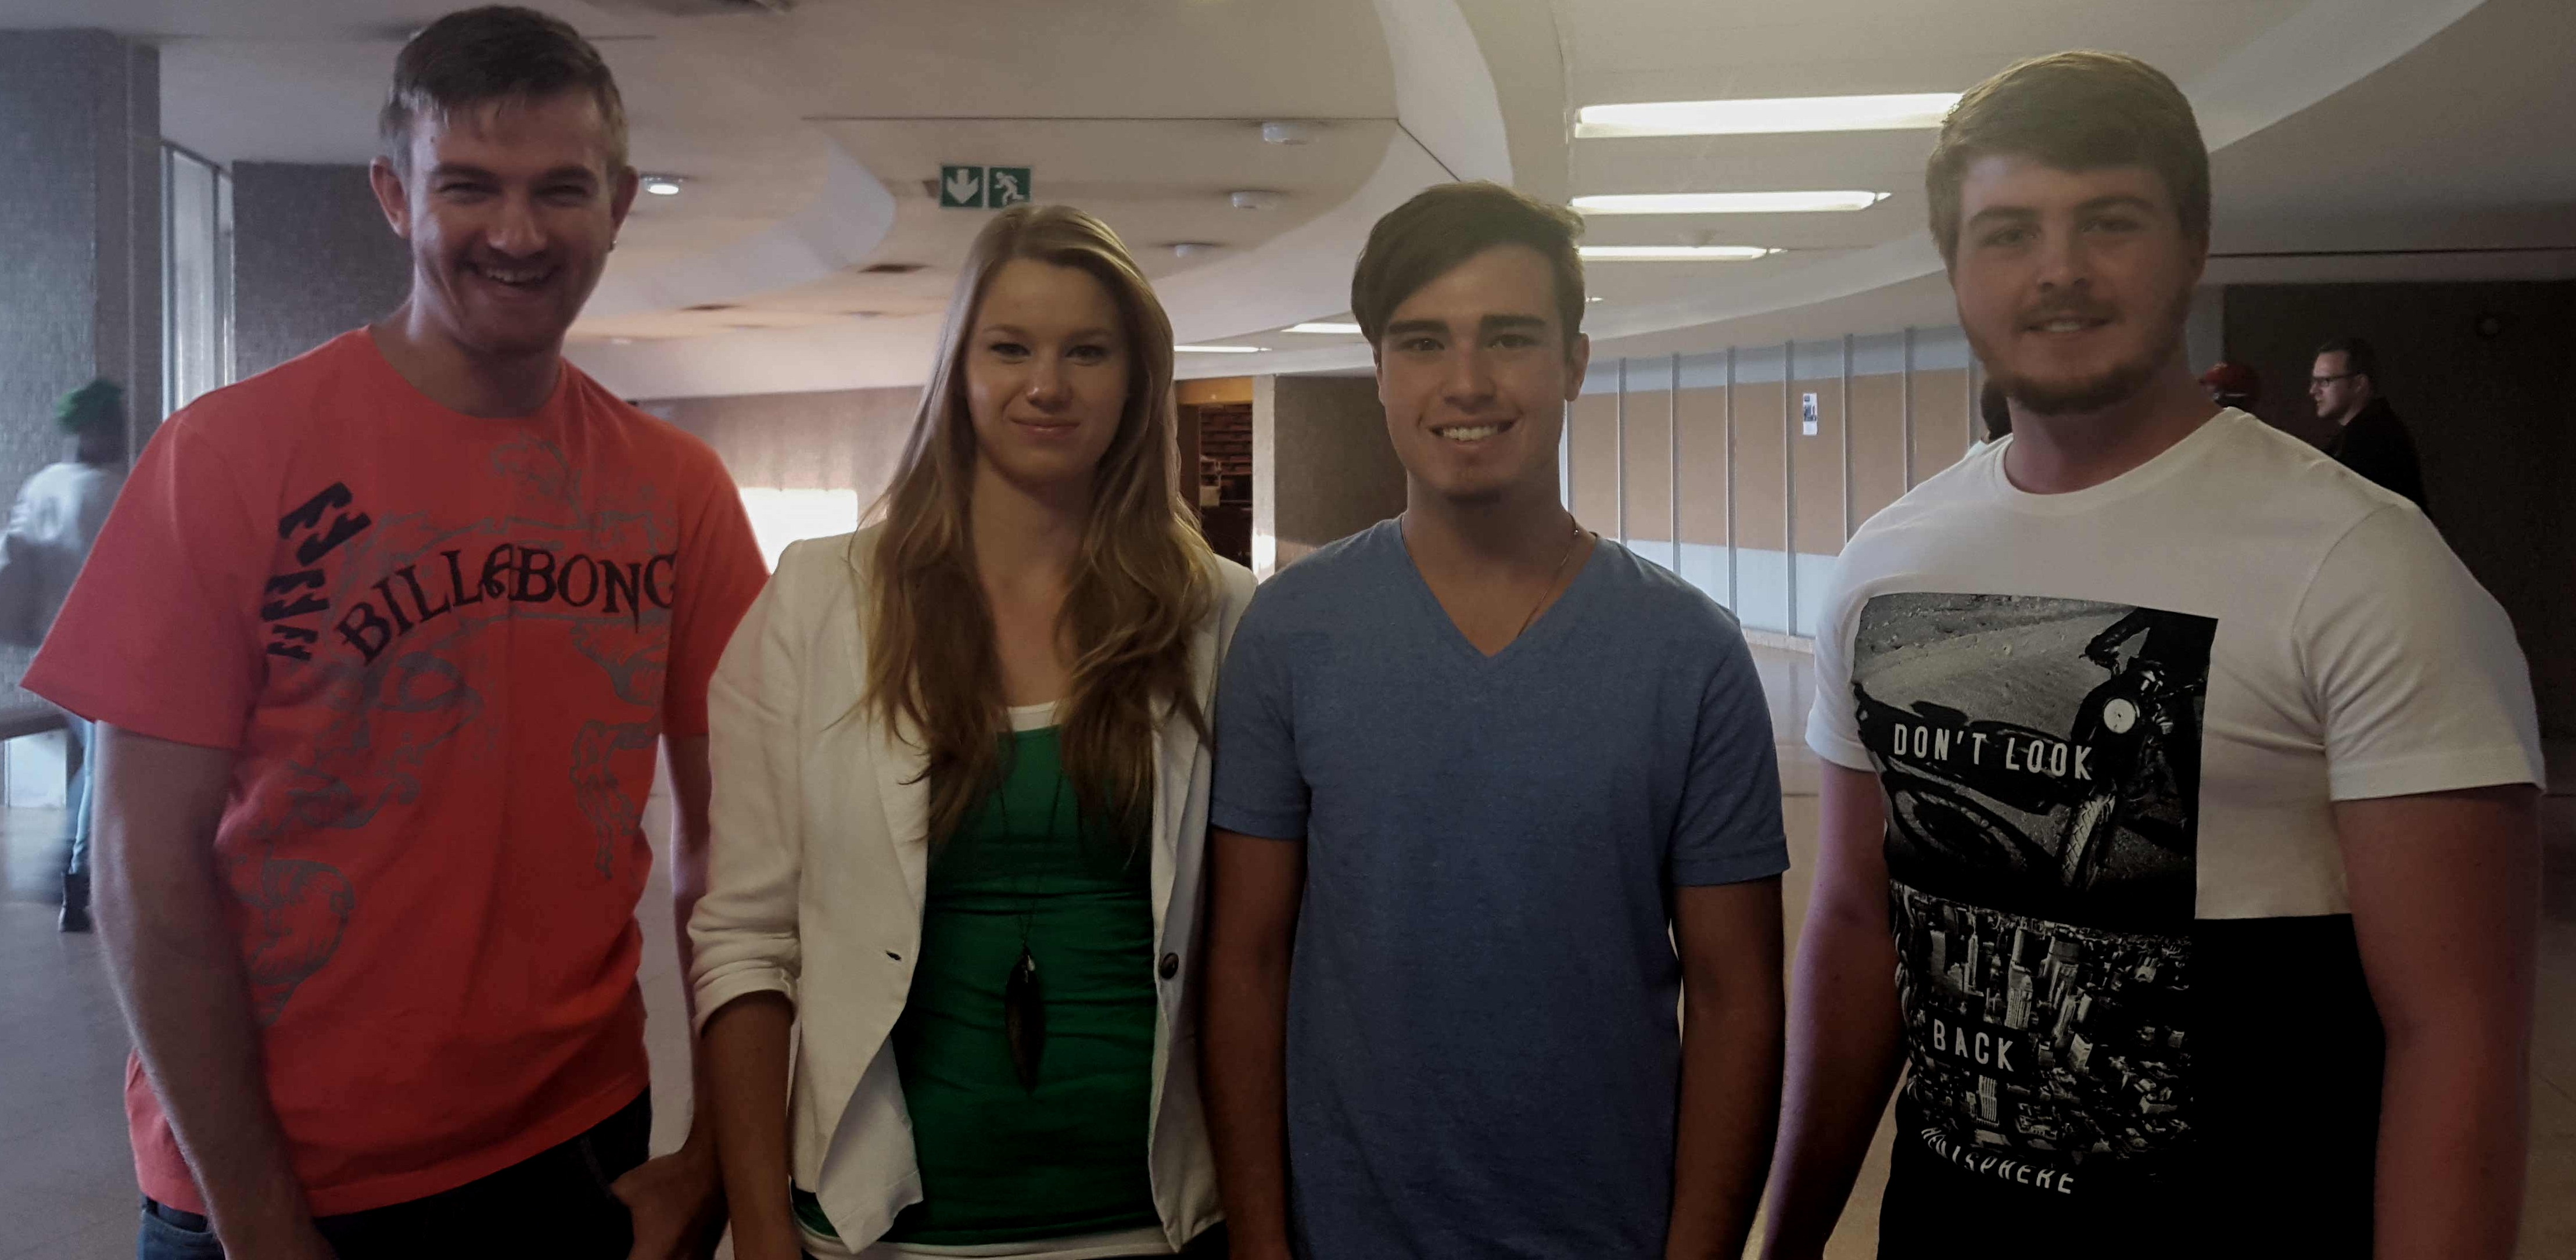
\includegraphics[width=\linewidth]{team.jpg}
			\end{figure}
		\end{center}
		\vspace*{\stretch{2.0}}
	\end{titlepage}
	\newpage
	\tableofcontents
	\newpage
	\pagenumbering{arabic}
	\section{The Team}
		\subsection{Nathan Dunkley}
		
		\subsection{Arno Grobler}
			\begin{wrapfigure}{l}{5.1cm}
				\begin{center}
					
\includegraphics[width=5cm]{arno.jpg}
				\end{center}
			\end{wrapfigure}
			\paragraph{Interests and Hobbies}
			My interests include collecting music, long distance running, painting and drawing, reading, computer games and obviously spending most of my days programming. Not only do I want to program as a profession, it is also a hobby for me. Integrating my other hobbies into my programming is my passion.
			
			\paragraph{Technical Skills}
            I pride myself in always looking for new skills and for me, learning a new technical skill is the best part of the experience. I enjoy making my projects look visually pleasing and spend as much time making a working, functional program as I do making it look good. I have good logical and problem solving skills and enjoy problems presented to me in computer science. My technical skills stem from Mathematics and computer science, especially those skills from data structures and algorithms and programming logic.
			
			\paragraph{Past Experience}
            I have created static websites for companies before, my most recent one is (\href{http://bodytalkbethlehem.com/}{http://bodytalkbethlehem.com/}) and (\href{http://honeydewpools.co.nf/}{http://honeydewpools.co.nf/}).
			
			\paragraph{Non-Technical Strengths}
			\begin{itemize}
				\setlength\itemsep{0.2em}
			        \item Eager learner
			        \item Organised 
			        \item Good time management
			        \item Good communication skills
			        \item Creative
			\end{itemize}
			
			\paragraph{Motivation}
			To do..
		
		\newpage
		\subsection{Amy Lochner}
		    \begin{wrapfigure}{l}{5cm}
				\begin{center}
					
\includegraphics[width=8cm, height=4.5cm, angle=90]{amy.jpg}
				\end{center}
			\end{wrapfigure}
			\paragraph{Interests and Hobbies}
			My interests include music, classic cars, cooking, traveling, breeding Shetland sheepdogs. My hobbies include reading, playing piano, camping, 4x4ing, tennis, training my dog, mountain biking and horse riding.
			
			\paragraph{Technical Skills}
			I am good at determining functional requirements of a system. I can place myself in the users shoes, this is valuable when determining how the user will intend to use a system. I can follow business logic easily and I have experience in databasing, Informatics, Statistics, Mathematics, multiple programming languages and Human Computer Interaction.
			
			\paragraph{Past Experience}
			I have built a fully functional, responsive website. I have helped a company modify their website. I have also observed (by job shadowing) the process of creating a system for a business and have noticed which qualities have caused them to excel and which have caused them to fail. I intend to use that knowledge to keep our team constantly progressing forward.
			
			\paragraph{Non-Technical Strengths}
			\begin{itemize}
				\setlength\itemsep{0.2em}
			        \item Organized
			        \item Good at prioritising 
			        \item Team player
			        \item Good leader
			        \item Optimistic
			        \item Quick learner
			        \item Determined
			\end{itemize}
			
			\paragraph{Motivation}
			To do..
		\newpage
		\subsection{Armand Maree}
			\begin{wrapfigure}{l}{5.1cm}
				\begin{center}
					
\includegraphics[width=5cm]{armand.jpg}
				\end{center}
			\end{wrapfigure}
			\paragraph{Interests and Hobbies}
			During my off time I like to socialize with friends and enjoy watching sports. I also like solving puzzles to keep my brain active during holidays.\\
			Tutoring scholars and university students has become a passion for me. I always look forward to these sessions.
			
			\paragraph{Technical Skills}
			I am good at solving complex problems and building data structures. I believe this is a valuable skill to complete any project, especially in the field of computer science.
			
			\paragraph{Past Experience}
			I have developed websites for other start up companies and I also have a website of my own (\href{http://www.codehaven.co.za}{www.codehaven.co.za}).
			I also have some Android developing experience I gained from side projects.
			
			\paragraph{Non-Technical Strengths}
			\begin{itemize}
				\setlength\itemsep{0.2em}
				\item Good leader
				\item Fast learner
				\item Team player
				\item Good communicator
			\end{itemize}
			
			\paragraph{Motivation}
			THIS SECTION IS PROJECT SPECIFIC
			
	\newpage
	\section{Project Execution}
\end{document}
